\documentclass{sigchi}

% Use this command to override the default ACM copyright statement
% (e.g. for preprints).  Consult the conference website for the
% camera-ready copyright statement.


%% BEGIN -- OVERRIDE THE DEFAULT COPYRIGHT STRIP
\toappear{
	
\includegraphics[scale=0.5]{assets/88x31.png}
	
    This work is licensed under the Creative Commons Attribution-ShareAlike
    4.0 International License. To view a copy of this license, visit\\
    {\url{http://creativecommons.org/licenses/by-sa/4.0/}}.
    {Copyright \copyright~2015}}
%% END -- OVERRIDE THE DEFAULT COPYRIGHT STRIP


% Arabic page numbers for submission.  Remove this line to eliminate
% page numbers for the camera ready copy

%\pagenumbering{arabic}

% Load basic packages
\usepackage{balance}  % to better equalize the last page
\usepackage{graphics} % for EPS, load graphicx instead
%\usepackage[T1]{fontenc}
\usepackage{txfonts}
\usepackage{times}    % comment if you want LaTeX's default font
\usepackage[pdftex]{hyperref}
% \usepackage{url}      % llt: nicely formatted URLs
\usepackage{color}
\usepackage{textcomp}
\usepackage{booktabs}
\usepackage{ccicons}
\usepackage{todonotes}
\usepackage{footnote}
\usepackage{mathptmx,helvet,courier}  \usepackage{array}
\usepackage{ragged2e}
\usepackage{tabularx,ragged2e,booktabs,caption}
% \usepackage{csquotes}
% \SetBlockEnvironment{quotation}% I've only added this
\newcolumntype{C}[1]{>{\Centering}m{#1}}
\renewcommand\tabularxcolumn[1]{C{#1}}
\usepackage{tablefootnote}
\usepackage{array}
\newcolumntype{P}[1]{>{\centering\arraybackslash}p{#1}}
\pagenumbering{arabic}
% llt: Define a global style for URLs, rather that the default one
\makeatletter
\def\url@leostyle{%
  \@ifundefined{selectfont}{\def\UrlFont{\sf}}{\def\UrlFont{\small\bf\ttfamily}}}
\makeatother
\urlstyle{leo}

% To make various LaTeX processors do the right thing with page size.
\def\pprw{8.5in}
\def\pprh{11in}
\special{papersize=\pprw,\pprh}
\setlength{\paperwidth}{\pprw}
\setlength{\paperheight}{\pprh}
\setlength{\pdfpagewidth}{\pprw}
\setlength{\pdfpageheight}{\pprh}

% Make sure hyperref comes last of your loaded packages, to give it a
% fighting chance of not being over-written, since its job is to
% redefine many LaTeX commands.
\definecolor{linkColor}{RGB}{6,125,233}
\hypersetup{%
    pdftitle={document},
    pdfauthor={},
    pdfkeywords={},
    bookmarksnumbered,
    pdfstartview={FitH},
    colorlinks,
    citecolor=black,
    filecolor=black,
    linkcolor=black,
    urlcolor=linkColor,
    breaklinks=true,
}

% create a shortcut to typeset table headings
% \newcommand\tabhead[1]{\small\textbf{#1}}

% End of preamble. Here it comes the document.
\begin{document}

\title{Extending StackOverflow® Gamification Using Social Media}

\numberofauthors{5}
\author{%
    \alignauthor{Arturo Reyes Lopez\\
        \affaddr{University of Victoria}\\
        \affaddr{Victoria, BC, Canada}\\
        \email{areyeslo@uvic.ca}}\\
    \alignauthor{Nitin Goyal\\
        \affaddr{University of Victoria}\\
        \affaddr{Victoria, BC, Canada}\\
        \email{ngoyal@uvic.ca}}\\
    \alignauthor{Richard B. Wagner\\
        \affaddr{University of Victoria}\\
        \affaddr{Victoria, BC, Canada}\\
        \email{rbwagner@uvic.ca}}\\
    \alignauthor{Tim Baker\\
        \affaddr{University of Victoria}\\
        \affaddr{Victoria, BC, Canada}\\
        \email{timbaker@uvic.ca}}\\
    \alignauthor{Alastair Beaumont\\
        \affaddr{University of Victoria}\\
        \affaddr{Victoria, BC, Canada}\\
        \email{alastair@uvic.ca}}\\
}

\maketitle

\begin{abstract}
\textbf{Gamification is the application of game playing elements (point scoring, competition, badges etc.) to other areas of activity to encourage engagement and participation. StackOverflow (SO) is a popular Q\&A community, with thousands of users solving and answering questions. SO uses badges and reputation metrics among other things to practice gamification.  The motivation for this project was to identify and measure the effectiveness of gamification on SO and to determine how it could be improved to facilitate engagement. We argue that inclusion of social media and classification of badges according to technical proficiencies could improve gamification. To conduct a qualitative analysis, surveys and interviews were directed. The first group of users for the survey were selected by sampling in a medium reputation range from the SO community and a second group was from students at the University of Victoria. The questions were revised and a proper random sampling was conducted. Interviews were then conducted for users belonging to different reputation levels. Analysis from the survey results and interviews showed that inclusion of social media and technical proficiency is not required. However, there is a need for the reputation system to be more meaningful on the whole.}
\end{abstract}


\keywords{Gamification, StackOverflow (SO)}

\category{H.5.m.}{Information Interfaces and Presentation (e.g. HCI)}{Miscellaneous} 

\pagebreak

\section{Introduction}
In Social Media, the use of game design and game elements, known as gamification, is used to increase the quality and quantity of user generated content. Badges, privileges and reputation are being used to recognize contributions of users on the sites and generally these elements seem to be valued by users who compete for some form of reward whether it be direct financial reward, the building of reputation, the recognition of skills, etc. Several studies have shown awareness of other participants and competence during the game experiences\cite{Rughinis}. Other studies have shown that gamification can increase engagement in activities that involve a community \cite{Marder}. However, the inclusion of gamification itself does not guarantee an increase in engagement or motivation. Its effectiveness depends on the rules dictating the aquasition of badges and privileges according to the context \cite{Deterding}.

StackOverflow (SO) is a popular Q\&A website for an ever-increasing range of computer programming topics and is among a larger network of similar sites branded and operated by Stack Exchange Inc.. SO is likely to be the most popular website in the computer programming world with just under five million registered users \footnote{https://stackoverflow.com/users} and with more than eleven million questions \footnote{https://stackoverflow.com/questions}. The website serves as a platform for users to both ask and answer questions related primarily to programming. These contributions by the users are the bulk of the content on the site and are met with reputation points and badges for the user. Our intention was to examine whether the use of gamification elements, such as the badges and points, were a primary motivating factor for the collaboration on the site. If so, we would determine areas for improvement in that current system in order to foster growth in the amount and quality of the user generated content and enable further collaboration from users that would not normally contribute to the site.

This research aims to determine in what ways the collaboration, in the form of asking, answering and commenting on questions, was achieved in the SO community.
Additionally, this research investigates what changes could be made to encourage more collaboration from users of all skill levels.

We hypothesized that the use of gamification elements on SO was an essential motivating factor for encouraging users to contribute. If this is true, we would like to examine whether aspects of the gamification can be improved upon to increase contributions to the site. We also believe that if users were given the option to share these elements (badges, reputation points, etc.) on certain social media platforms, that there would be an increase in contribution from users. We will gather input from current users as to how and where they would like to be able to share the gamification elements or adversely why they may not want to share these elements. During the survey and interview stages of our research we hope to gather sufficient evidence to affirm or negate these hypotheses.

Throughout our research, we presented an overview of relevant related work, examining what the primary motivating factors are for user collaborations. We will discuss the merits and shortcomings of the current system and provide recommendations of how SO may be improved upon to encourage more active participation from a wider range of its users.


\section{Related work}

The vast majority of SO users only post once and are seen as a nuisance by other users as they do not provide quality content to the website or 'upvote' the users that answer their questions \cite{Slag}. These users are more likely to not have their questions answered because the new users tend to ignore them by not providing them with reputation (by upvoting). New users are also more likely to recieve negative feedback or answers that can be interpreted as negative feedback. This causes a gap between new users and the other more experienced users because of the commonly held view that new users will not contribute and make the community negative and unfriendly. This lack of cohesion between low and medium reputation level users raises a question of whether gamification works \cite{Hamari}. The research in this paper indicates that gamification on SO facilitates more posting, however, the effects are greatly dependent on the context in which gamification is being implemented. The gamification rewards users who work hard to gain badges and reputation in the context of increasing social capitol and not material benefits. 

A heavy majority of users look to build their reputation in SO and the best way to accomplish this is by posting on trending topics such as .NET technologies, Object orientated programming languages and web development \cite{Bosu}. The dynamics of reputation building also rely on the time of posting, the skills and effort put into a post by the reputation seeker. Therefore, expertise in tranding topics is a must to gain reputation quickly. These reputation seekers should also participate regularly and answer as many questions as possible. All these actions will help improve a contributor's chance of getting up-votes to increase their reputation.  This reputation seeking attitude also has a correlation to commits on GitHub \cite{Vasilescu}. This link between the two platforms (SO and GitHub) can catalyze committing on GitHub from active committers who answer questions on SO. These users looking to increase their reputation will also change their behavior to achieve badges \cite{Wang}.  Shaowei et al. talked about the different actions to increase reputation, such as editing posts, asking and answering questions and discovered the users who receive a badge for asking questions are not motivated to earn more badges. These authors proposed an anonymous question feature to increase the rate of posted questions. However, they hypothesised the inclusion of an anonymous question feature could decrease the quality and increase the number of questions on SO. This research brings up questions of how Q/A platforms deals with the toxicity that sometimes disturbs content creation and motivation.

Cavusoglu et al. analysed the answering behaviour from a dataset with 46,571 SO users. The analysis revealed a positive impact on increasing the number of answers due to badges \cite{Cavusoglu}. The study focused on comparing the answering activity 7 days before getting a badge and 7 days after the awarding date. They assessed the extent to which users are encouraged by gained badges in there answering activity. The analysis was more focused on the behaviour of members after receiving a badge. In general, the researchers have shown that badges motivate the participation of the user. However, we argue that the inclusion of programming skills or technical proficiency to the current classification of badges, besides sharing achievements on social media, could boost an increase of participation in SO.


\section{Research Methodology}
To study the collaboration in SO in the form of asking, answering and commenting on questions, we set up a qualitative framework to research the human aspects of SO with the motivation to increase the contributions from the community \cite{Easterbrook}. Several methodologies can be applied to carry out the research: controlled experiments, case study, ethnographies or survey research. A case study has its limitations such as to not capture the real motivation and therefore is not appropriate in this research. A controlled experiment is not applicable as we do not have enough information in advance about the control variables and our research questions are focussed on the proposing an improved design for gamification elements to foster contribution. Ethnographic research does not seek to prove hypotheses and theories and our research focuses on proving the hypotheses initially formulated to improve gamification \cite{Easterbrook}.


In this research, we chose surveys and interviews as the empirical approaches to gather the data and the motivation to contribute on SO. The research was divided into three data collection phases: pilot surveys, exploratory surveys followed by interviews. The answers collected from the surveys can provide us with general insights towards testing our hypotheses. The interviews were carried out based on the email addresses provided to us by the participant of the exploratory survey. The interviews provided us the opportunity to clarify and to deepen patterns which emerged by the reputation level in the analysis of the survey responses.

\subsection{Research Questions}
The interest of sharing badges and reputation on Social Media has been shown in the community through previous years \footnote{http://meta.stackexchange.com/questions/141300/how-can-i-share-my-stack-overflow-reputation-on-facebook} and we believe that social media can reinforce the current gamification as external factor. In addition, we argue that current gamification can be improved through including programming language as the means of classifying earn badges by the user. As follows, we include the research questions to approach the experiment:

\textbf{How does the current gamification used by StackOverflow need to be improved in order to meet the user requirements?}

This question will provide us the possible dissatisfaction in the user experience related to gamification and find the possible improvements on current classification of badges. The result will involve a change on how the badges are being classified to more suitable classification including more detailed characteristics such as programming language.

\textbf{Is the publication of reputation and badges on social media a
factor to promote more answers?}

This question will explore the user reaction when sharing reputation and badges on social media such as Facebook, Twitter or Linked-in. We will study if this additional recognition can stimulate the contributions in the community.

\textbf{How would users like to use their reputation and badges
on social media and alike?}

This question will provide us the vision about the specific information that the users would like to share on social media. The users can provide recommendation on how they would like to export their achievements to other social media platforms and which information they would consider to be shareable.

\subsection{Study Design}
Our research design consisted of two main phases namely surveys and interviews. For both the phases, our research included two groups of users: SO members classified by reputation level and University of Victoria student population. The basic information of SO members was retrieved from the data dump hosted \footnote{https://data.stackexchange.com/stackoverflow/query}by SO. However, in the previous year, SO has removed the email contact from the databases to protect member's privacy \footnote{http://meta.stackexchange.com/questions/221027/where-did-emailhash-go}.Therefore, we obtained the emails by extracting them from their GitHub account. Most of the users who have SO account also have it linked with their GitHub account. A web crawler script was developed to map the users from SO to their GitHub accounts to retrieve the email address for GitHub. After gathering the SO members emails, we realized that members with low-level reputation usually do not have their GitHub account linked. However, University of Victoria student population provide us the means of obtaining the insights of the low-reputation-level users who look on SO for obtaining answers related to predefined questions by SO members. Ultimately, University of Victoria students were excluded from the quantitative study. The research is limited from the fact that the users who have there accounts linked to GitHub belongs to medium and high reputation level which makes the purposive sampling shifts towards these reputation levels.

The reputation level in SO follows an approximately exponential distribution with a long tail as is shown \footnote{http://hewgill.com/\~greg/stackoverflow/stats.html}. As a result, we sampled in clusters on a logarithmic scale (e.g. 0-9, 10-99, 100 - 999, 1,000 - 9,999 and 10,000 - infinite) and sent bulk emails including the survey questionnaire to each group. In the University of Victoria student group, we assumed to obtain members mostly from the first reputation interval.

In the first two phases, we sent a pilot and exploratory survey by email consisting of 13 questions to cover 4 features to be studied: Period of time using SO and activities in the community, the motivation to contribute through answering questions, behaviour towards sharing reputation on social media and possible changes in badges classification. In the email, we attached the consent form explaining the characteristics of the research and rights of participants involved. In the third phase, interviews were included to complement the qualitative research and overcome the limitations of general answers in the surveys. The questionnaire for interviews provided us the opportunity to increase our understanding of the preliminary results obtained by the surveys. Therefore, some questions in the interviews were personalized according to the reputation level of the user to be interviewed. For SO members, the interviews were held on Skype and face-to-face for University of Victoria student population, the interviews lasted between 30 to 40 minutes and  scheduled based on the availability of the interviewee. The interviewer asked for permission to record the interview while taking notes. In some cases, the interviewer deviated from the rewritten questions to get more insightful results.


The insight of having three different phases provided us the opportunity to clarify some behaviour presented in the answers when analyzing the survey. The survey form was sent to 551 participants in total distributed among all reputation levels and we obtained 72 responses (13.07\%) from those 5 members (0.9\%) were willing to participate in an interview. Table 1 shows the participation of members classified by their reputation level and the number of members from each group who provided us with interviews.

\begin{center}
    \begin{tabular}{ | p{1.0cm} | p{1.6cm} | P{0.9cm} | P{1.8cm} | P{1.4cm} |}
    \hline
    \textbf{Group ID} & \textbf{Reputation Level} & \textbf{Emails Sent} & \textbf{Survey Participation(\%)} & \textbf{Interview Participation } \\ \hline
    G1 & 0-9 & 43 & 2.3\% & 1 \\ \hline
    G2 & 10-99 & 69 & 13.0\% & 0 \\ \hline
    G3 & 100-999 & 144 & 13.0\% & 1 \\ \hline
    G4 & 1,000-9,999 & 146 & 17.0\% & 2 \\ \hline
    G5 & 10,000-inf. & 149 & 12.0\% & 1 \\ \hline
  \end{tabular}
   Table1.Responses on surveys/interviews.
\end{center}

\pagebreak

\section{Findings}

The following section includes the results from the surveys and interviews based on the research questions.To study the current gamification in SO, we included three important research questions: what is the motivation to contribute, how much satisfaction is there with the current gamification and how the member would like to improve the current gamification.

\textbf{RQ1. How does current gamification used by StackOverflow need to be improve in order to meet the user requirements?}

At the inception of the project, based on the discussion with our team we hypothesized that current gamification in SO community can be improved. The badges and reputation currently provided by SO are static and non-exportable to resumes or personal websites. We took a pragmatic decision to include this question on the survey to identify if there is a definite need to improve the gamification elements in SO community and if it is then how can it be improved further.

From the analysis of the responses we found that the main motivation to contribute on SO can vary according to the user reputation level. For example, the lowest reputation level is more interested on increasing their knowledge through asking questions. The medium reputation levels are more appealing to contribute on SO when applying their experience while building reputation. On the other hand, the highest reputation level is more focused on applying experience while challenging themselves with unusual questions. One answer from an interview can clarify this aspect :

\begin{quote}
Only if the question is interesting and deep enough for me, I would consider answering it, if it is not interesting or deep enough for me, I am not saying I am a good programmer, it’s only my personal taste. --- (G4P1)
\end{quote}

Surprisingly, when asking about how satisfied members are with the current gamification, the lower reputation levels (0-9,10-99) are more satisfied than the higher reputation levels.A user from group G3 said that
\begin{quote}
It is good and it is already motivating and encouraging. Only the pace for earning badges is low as SO community is strict for new users, it was easy previously but it is harder now to earn badges for a new user. -- (G3P1)
\end{quote}


On the other hand, the higher  reputation levels (100-999, 1,000-9,9999 and more than 10,000) are dissatisfied with the current gamification.  These results suggest that new users are attracted for the current use of badges and reputation while users with more experience do not see as much value in them. An answer from our interviews can provide us more insight about this phenomenon:

\begin{quote}
If a fresh person wants to start participating, asking, answering, then yes I agree that badges would play an important role in incentivize participation, ...when a newcomer would pay attention to those gamifications objects because he would know how StackOverflow works, he would know by that time that badges mean nothing. --- (G4P1)
\end{quote}

Overall, about two-fifths of respondents at all reputation levels agreed that sharing reputation and badges on GitHub as a feature would increase their contributions in the community. In our interviews, we found the same relationship between SO and GitHub, but in the other way round:

\begin{quote}
Sharing GitHub on StackOverflow would made, increase the incentive to motivation to answer or ask question if they see the GitHub profile. --- (G4P1)
\end{quote}

Another interesting perspective we infer from the highest level user G5P1 is that the current gamification does not reflect the current expertise of a user. He said 
\begin{quote}
The tag badges that I am criticising a bit because once you have reached a 1000 points and 200 questions you do not have enough indication about the [expertise of the user] --- (G5P1).
\end{quote}

Through the interview with G4P1 we observed a sense of devalued reputation and value of badges in SO.

\textbf{RQ2. Is the publication of reputation and badges on social media a factor to promote more answers?}

At the beginning of the exploratory study, we discussed that the inclusion of Social Media on SO would increase the participation or the motivation to contribute through sharing reputation or badges to a broader community. This social media sharing aspect could even be repurposed to the work-related community such as GitHub, Linkedin or Twitter. We unfolded this question into two perspectives: How can the ability to share achievements on Social Media can affect the contributions and which Social Media platforms would be preferred by the users of said sites.

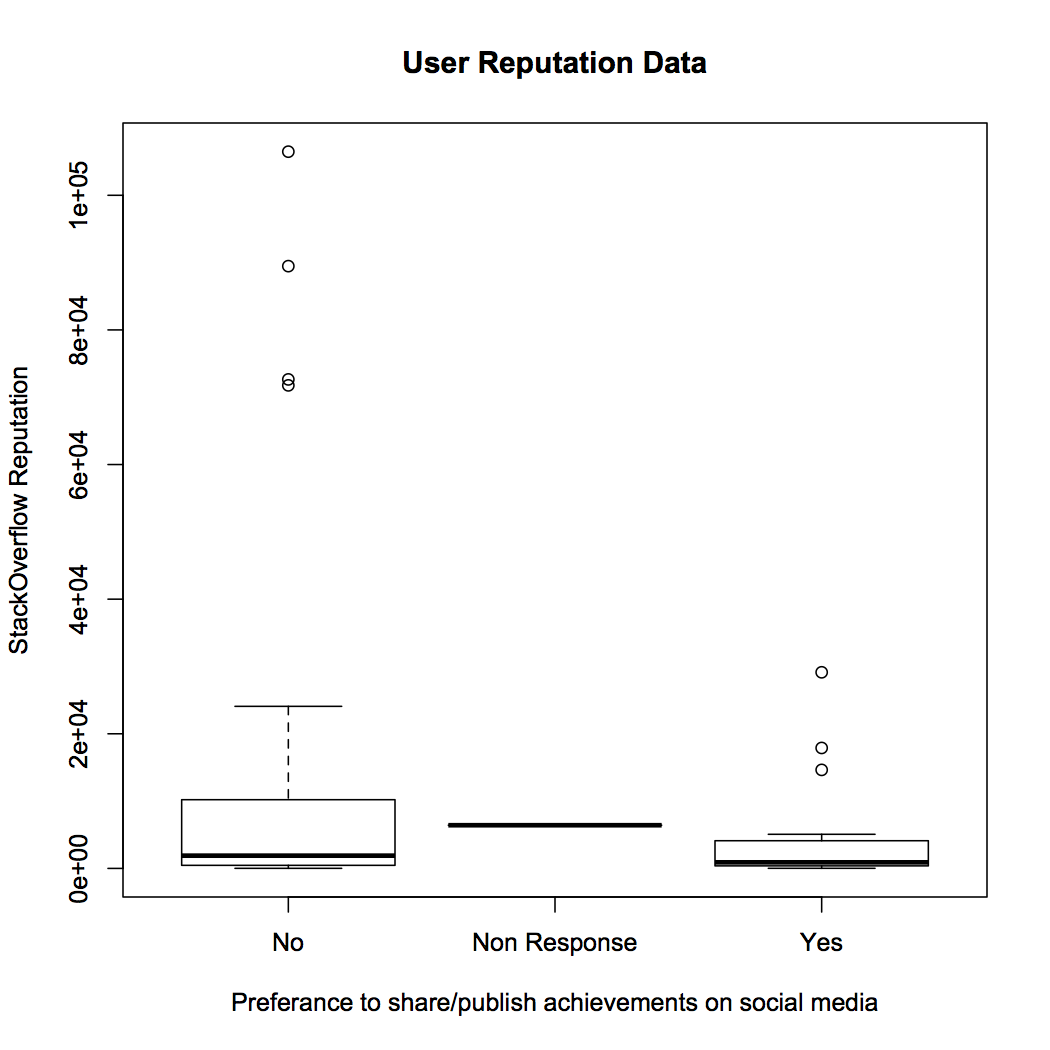
\includegraphics[scale=0.5]{figures/boxplot_reputation_compare_publish_reputation_bool.png}

The graphic above shows a general trend that was found in the surveys and the interviews where more acclimated users didn't find value in self reported motivation from the badges. On the other hand, less acclimated users (generally with lower reputation) were slightly more likely to find value in the badges.

From the interviews, a user from the reputation level 1,000-9,999 provided us an interesting justification for not sharing his badges and reputation on GitHub: 
\begin{quote}
GitHub in my opinion is the only popular place where you can really show your skills, so answering your question, sharing StackOverflow badges on GitHub would do nothing. --- (G4P1)
\end{quote}
and not sharing in LinkedIn: 
\begin{quote}
LinkedIn is in my opinion a place where headhunters live, not a place to share your achievements because you don’t find a soul mate who appreciate your achievement. --- (G4P1)
\end{quote}
Another member with the highest reputation level in our sample says that
\begin{quote}
 If they (medium level users) are still there (SO) just for badges and reputation then maybe they are there for wrong reasons. --- (G5P1)
 \end{quote}
 
The members who agreed to share their achievements on Social Media preferred LinkedIn (91\%), Twitter (78\%) and Facebook (56\%). The answer to the question, how does your contribution will be affected if SO start to share your reputation and badges, confirms the interest of the lower reputation groups to increase their motivation. On the other side, the other reputation levels  do not agree with the this sentiment. Overall, we did not find enough evidence that Social Media can improve the current gamification. In fact, it is the use of badges among those acclimated to the community seems a point of contention probably worth studying on its own.

\textbf{RQ3. How would users like to include their reputation and badges on social media?}

As the part of preliminary analysis of the research question, we found evidence of people wanting to include their reputation and badges from SO to social media \footnote{http://meta.stackexchange.com/questions/141300/how-can-i-share-my-stack-overflow-reputation-on-facebook}. Based on the discussion with the team, we suggested few ways in which the reputation and badges can be included/exported on social media. Our suggestion came from a careful discussion based on the usability and functionality. We suggested to separate the badges on programming language as the current badges interface does not provide enough information about in which domain or technical proficiency it was awarded for. The results show that lower reputation users agree to include programming language classification in the badges while higher reputation users do not. The higher reputation users seem to have more justifications about the nonconformity of the current gamification. An interview provided us with  a better insight about this:

\begin{quote}
The process of earning reputation should be [scaled] exponentially [in terms of] difficult[y]. If you get at the level A and then you answer twice [as] many questions after level A, you wouldn’t get twice reputation than you got before level A, it should be exponentially difficult, the curve should not be flat. --- (G4P1)
\end{quote}

We can identify a necessity of changing the means by which assignment of  badges and reputation among the different reputation levels takes place.

Another interesting aspect we discovered while conducting our interviews was this concept of a tutorial. Even though this does not relate to our research questions, the idea brings up further points about incentivizing users to post. During the interview of a low reputation user, a main issue with a lack of posting was correlated to a lack of stimuli from SO. This user suggested implementing helpful tips or a tutorial option in which SO would gently prompt users about features of the website and help them learn the tools at their disposal while simultaneously build up reputation. The use of a non-disruptive tutorial to teach users mechanics is very similar to a parallel in video games where users are taught how to manipulate their avatar one step at a time. If SO could find the same balance of creating a tutorial that is helpful but not disruptive like popular video games have in the past, this would dramatically increase the input from these low reputation users and could even be a useful medium to convey new site mechanics to medium and high reputation users.


\section{Limitations}

Our study was primarily designed to investigate the strengths and shortcomings of the SO reputation system with assumptions that the reputation system was somewhat effective. We hypothesised the possibility to make reputation system more valid by exporting it to other platforms similar to how gaming platforms allow for the sharing of achievements to habituate completionist\footnote{A player (of a game) who attempts to fully complete the game unlocking all achievements and trophies} behaviour. What was found was that the reputation system is deeply flawed and our initial assumptions were lacking. This made some of the questions we asked biased in the direction of favouring the reputation system. Part of the problem that instigated this was a lack of literature on the subject of gameification especially when concerned with social media integration. 

We quickly ran into problems in our approach of sampling the users (in clusters) on SO and our results were skewed. This stems from fundamental design decisions in the inception. We now hypothesis that the lower reputation users (G1, G2) were less keen to respond to our survey for reasons of a lack of expertise of SO. Additionally, the lower reputation users had a lower rate of connection with GitHub account which was essential to our method of correspondence. 


\section{Future Work}

A logical next step would be to do a follow-up study investigating actual user behaviour as appose to self-reported behaviour from this study with the intention of finding heuristics that predict expertise as appose to participation. This could be done with some effort by using the SO posting statistics and combining them with the user data. 


\section{Conclusion}

After compiling the results from the survey and with much consideration to the interviews, we have isolated some trends that look to be convincing. We found that our research questions did not cut deep enough into the issue of gamification on SO. From both the interviews and the survey, it became clear that unacclimated users value the reputation much more then established users.

After analyzing the results obtained from the survey and interviews, we are convinced there is a need to improve the current gamification elements SO operates with. The results from this study imply that the gamification elements on SO are not very effective at motivating acclimated users. Using a different mechanism for badge and reputation acquisition could potentially solve this problem. Further improvements to gamification in the core principles are needed before considering adding external features that would export the SO reputation system to other platforms. This may be important for not only SO but any platform that uses a reputation system for users which is becoming increasingly popular amongst newer sites as they become more weary of the quality of user submitted content.






% REFERENCES FORMAT
% References must be the same font size as other body text.
% \bibliographystyle{SIGCHI-Reference-Format}
% \bibliography{document}

\begin{thebibliography}{9}

\bibitem{Antin}
Antin, Judd, and Elizabeth F. Churchill. "Badges in social media: A social psychological perspective." CHI 2011 Gamification Workshop Proceedings (Vancouver, BC, Canada, 2011). 2011.

\bibitem{Bosu}
Bosu, Amiangshu, et al. "Building reputation in stackoverflow: an empirical investigation." Proceedings of the 10th Working Conference on Mining Software Repositories. IEEE Press, 2013.

\bibitem{Caponetto}
Caponetto, Ilaria, Jeffrey Earp, and Michela Ott. "Gamification and Education: A Literature Review." ECGBL2014-8th European Conference on Games Based Learning: ECGBL2014. Academic Conferences and Publishing International, 2014.

\bibitem{Cavusoglu}
Cavusoglu, Huseyin, Zhuolun Li, and Ke-Wei Huang. "Can Gamification Motivate Voluntary Contributions?: The Case of StackOverflow Q\&A Community." Proceedings of the 18th ACM Conference Companion on Computer Supported Cooperative Work \& Social Computing. ACM, 2015.

\bibitem{Deterding}
Deterding, Sebastian, et al. "Gamification. Using game-design elements in non-gaming contexts." CHI'11 Extended Abstracts on Human Factors in Computing Systems. ACM, 2011.

\bibitem{Easterbrook}
Easterbrook, Steve, et al. "Selecting empirical methods for software engineering research." Guide to advanced empirical software engineering. Springer London, 2008. 285-311.

\bibitem{Jin}
Jin, Yong, et al. "Quick Trigger on Stack Overflow: A Study of Gamification-influenced Member Tendencies." , 1916.

\bibitem{Marder}
Marder, Andrew. "Stack overflow badges and user behavior: an econometric approach." Proceedings of the 12th Working Conference on Mining Software Repositories. IEEE Press, 2015.

\bibitem{McGonigal}
McGonigal, Jane. "Reality is broken: Why games make us better and how they can change the world." Penguin, 2011.

\bibitem{Hägglund}
Hägglund, Per. "Taking gamification to the next level.", 2012.

\bibitem{Hamari}
Hamari, Juho, Jonna Koivisto, and Harri Sarsa. "Does gamification work?--a literature review of empirical studies on gamification." System Sciences (HICSS), 2014 47th Hawaii International Conference on. IEEE, 2014.

\bibitem{Rughinis}
Rughinis, Razvan. "Gamification for productive interaction: Reading and working with the gamification debate in education." Information Systems and Technologies (CISTI), 2013 8th Iberian Conference on. IEEE, 2013.

\bibitem{Ryan}
Ryan, Richard M., C. Scott Rigby, and Andrew Przybylski. "The motivational pull of video games: A self-determination theory approach." Motivation and emotion 30.4 (2006): 344-360.

\bibitem{Slag}
Slag, Rogier, Mike de Waard, and Alberto Bacchelli. "One-day flies on StackOverflow."

\bibitem{Vasilescu}
Vasilescu, Bogdan, Vladimir Filkov, and Alexander Serebrenik. "StackOverflow and GitHub: associations between software development and crowdsourced knowledge." Social Computing (SocialCom), 2013 International Conference on. IEEE, 2013.

\bibitem{Wang}
Wang, Shaowei, David Lo, and Lingxiao Jiang. "An empirical study on developer interactions in StackOverflow." Proceedings of the 28th Annual ACM Symposium on Applied Computing. ACM, 2013.


\end{thebibliography}

\end{document}

%%% Local Variables:
%%% mode: latex
%%% TeX-master: t
%%% End:
